\documentclass[14pt]{extbook}
\usepackage{multicol, enumerate, enumitem, hyperref, color, soul, setspace, parskip, fancyhdr} %General Packages
\usepackage{amssymb, amsthm, amsmath, latexsym, units, mathtools} %Math Packages
\everymath{\displaystyle} %All math in Display Style
% Packages with additional options
\usepackage[headsep=0.5cm,headheight=12pt, left=1 in,right= 1 in,top= 1 in,bottom= 1 in]{geometry}
\usepackage[usenames,dvipsnames]{xcolor}
\usepackage{dashrule}  % Package to use the command below to create lines between items
\newcommand{\litem}[1]{\item#1\hspace*{-1cm}\rule{\textwidth}{0.4pt}}
\pagestyle{fancy}
\lhead{Progress Quiz 4}
\chead{}
\rhead{Version B}
\lfoot{5346-5907}
\cfoot{}
\rfoot{Summer C 2021}
\begin{document}

\begin{enumerate}
\litem{
Construct the lowest-degree polynomial given the zeros below. Then, choose the intervals that contain the coefficients of the polynomial in the form $ax^3+bx^2+cx+d$.\[ \frac{-5}{3}, \frac{3}{5}, \text{ and } \frac{-4}{3} \]\begin{enumerate}[label=\Alph*.]
\item \( a \in [42, 46], b \in [107, 114], c \in [12, 24], \text{ and } d \in [-67, -56] \)
\item \( a \in [42, 46], b \in [-42, -40], c \in [-92, -85], \text{ and } d \in [59, 61] \)
\item \( a \in [42, 46], b \in [9, 14], c \in [-111, -107], \text{ and } d \in [-67, -56] \)
\item \( a \in [42, 46], b \in [-114, -106], c \in [12, 24], \text{ and } d \in [59, 61] \)
\item \( a \in [42, 46], b \in [107, 114], c \in [12, 24], \text{ and } d \in [59, 61] \)

\end{enumerate} }
\litem{
Describe the zero behavior of the zero $x = 6$ of the polynomial below.\[ f(x) = -3(x + 5)^{10}(x - 5)^{7}(x - 6)^{12}(x + 6)^{9} \]\begin{enumerate}[label=\Alph*.]
\begin{multicols}{2}\item 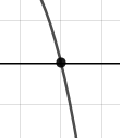
\includegraphics[width = 0.3\textwidth]{../Figures/polyZeroBehaviorAB.png}\item 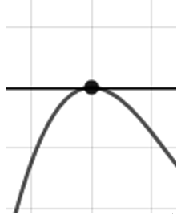
\includegraphics[width = 0.3\textwidth]{../Figures/polyZeroBehaviorBB.png}\item 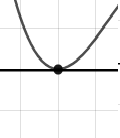
\includegraphics[width = 0.3\textwidth]{../Figures/polyZeroBehaviorCB.png}\item 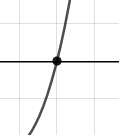
\includegraphics[width = 0.3\textwidth]{../Figures/polyZeroBehaviorDB.png}\end{multicols}\item None of the above.
\end{enumerate} }
\litem{
Construct the lowest-degree polynomial given the zeros below. Then, choose the intervals that contain the coefficients of the polynomial in the form $x^3+bx^2+cx+d$.\[ 4 - 5 i \text{ and } -2 \]\begin{enumerate}[label=\Alph*.]
\item \( b \in [1, 2], c \in [6, 8], \text{ and } d \in [9, 16] \)
\item \( b \in [6, 8], c \in [22, 31], \text{ and } d \in [-87, -77] \)
\item \( b \in [1, 2], c \in [-8, 5], \text{ and } d \in [-12, -6] \)
\item \( b \in [-6, -2], c \in [22, 31], \text{ and } d \in [75, 87] \)
\item \( \text{None of the above.} \)

\end{enumerate} }
\litem{
Which of the following equations \textit{could} be of the graph presented below?
\begin{center}
    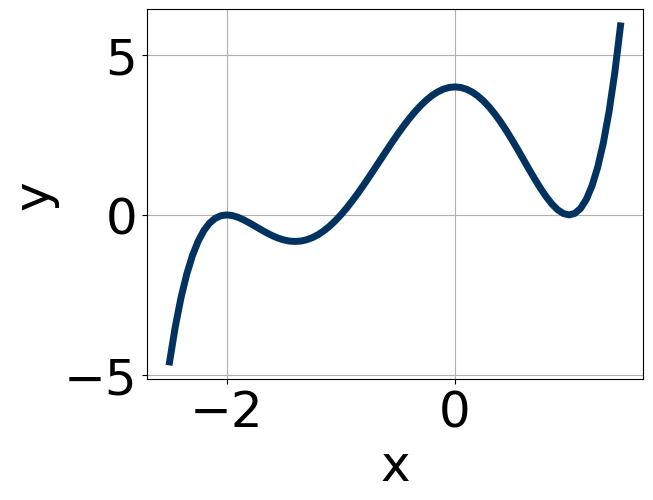
\includegraphics[width=0.5\textwidth]{../Figures/polyGraphToFunctionCopyB.png}
\end{center}
\begin{enumerate}[label=\Alph*.]
\item \( -8(x + 2)^{10} (x - 1)^{6} (x + 1)^{8} \)
\item \( 10(x + 2)^{6} (x - 1)^{6} (x + 1)^{5} \)
\item \( -15(x + 2)^{6} (x - 1)^{4} (x + 1)^{9} \)
\item \( 5(x + 2)^{10} (x - 1)^{11} (x + 1)^{7} \)
\item \( 15(x + 2)^{10} (x - 1)^{9} (x + 1)^{6} \)

\end{enumerate} }
\litem{
Describe the zero behavior of the zero $x = -6$ of the polynomial below.\[ f(x) = -9(x - 6)^{9}(x + 6)^{14}(x + 3)^{4}(x - 3)^{6} \]\begin{enumerate}[label=\Alph*.]
\begin{multicols}{2}\item 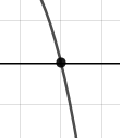
\includegraphics[width = 0.3\textwidth]{../Figures/polyZeroBehaviorCopyAB.png}\item 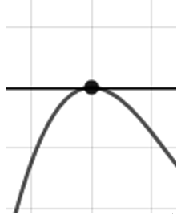
\includegraphics[width = 0.3\textwidth]{../Figures/polyZeroBehaviorCopyBB.png}\item 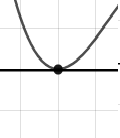
\includegraphics[width = 0.3\textwidth]{../Figures/polyZeroBehaviorCopyCB.png}\item 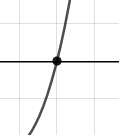
\includegraphics[width = 0.3\textwidth]{../Figures/polyZeroBehaviorCopyDB.png}\end{multicols}\item None of the above.
\end{enumerate} }
\litem{
Which of the following equations \textit{could} be of the graph presented below?
\begin{center}
    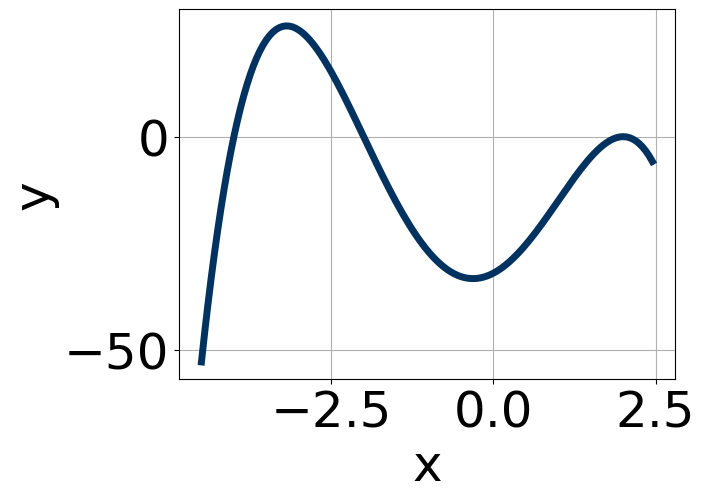
\includegraphics[width=0.5\textwidth]{../Figures/polyGraphToFunctionB.png}
\end{center}
\begin{enumerate}[label=\Alph*.]
\item \( 13(x - 2)^{8} (x + 2)^{11} (x + 4)^{10} \)
\item \( 4(x - 2)^{6} (x + 2)^{5} (x + 4)^{9} \)
\item \( -12(x - 2)^{10} (x + 2)^{8} (x + 4)^{7} \)
\item \( -14(x - 2)^{7} (x + 2)^{4} (x + 4)^{9} \)
\item \( -11(x - 2)^{6} (x + 2)^{11} (x + 4)^{7} \)

\end{enumerate} }
\litem{
Construct the lowest-degree polynomial given the zeros below. Then, choose the intervals that contain the coefficients of the polynomial in the form $x^3+bx^2+cx+d$.\[ -5 + 4 i \text{ and } -3 \]\begin{enumerate}[label=\Alph*.]
\item \( b \in [-7, 6], c \in [1, 11], \text{ and } d \in [8, 23] \)
\item \( b \in [-7, 6], c \in [-6, 2], \text{ and } d \in [-15, -11] \)
\item \( b \in [-22, -12], c \in [69, 77], \text{ and } d \in [-125, -114] \)
\item \( b \in [10, 21], c \in [69, 77], \text{ and } d \in [115, 125] \)
\item \( \text{None of the above.} \)

\end{enumerate} }
\litem{
Describe the end behavior of the polynomial below.\[ f(x) = 2(x + 9)^{3}(x - 9)^{8}(x + 5)^{3}(x - 5)^{4} \]\begin{enumerate}[label=\Alph*.]
\begin{multicols}{2}\item 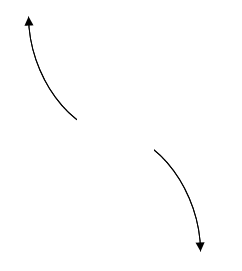
\includegraphics[width = 0.3\textwidth]{../Figures/polyEndBehaviorCopyAB.png}\item 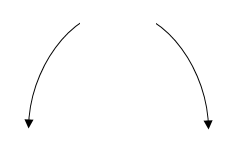
\includegraphics[width = 0.3\textwidth]{../Figures/polyEndBehaviorCopyBB.png}\item 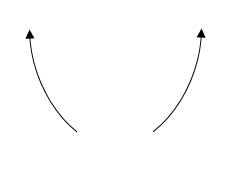
\includegraphics[width = 0.3\textwidth]{../Figures/polyEndBehaviorCopyCB.png}\item 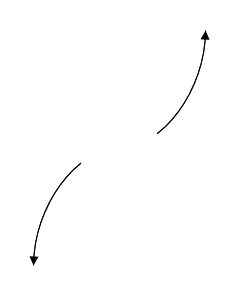
\includegraphics[width = 0.3\textwidth]{../Figures/polyEndBehaviorCopyDB.png}\end{multicols}\item None of the above.
\end{enumerate} }
\litem{
Describe the end behavior of the polynomial below.\[ f(x) = -7(x - 4)^{5}(x + 4)^{6}(x - 5)^{4}(x + 5)^{6} \]\begin{enumerate}[label=\Alph*.]
\begin{multicols}{2}\item 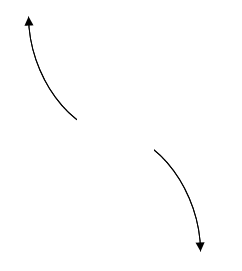
\includegraphics[width = 0.3\textwidth]{../Figures/polyEndBehaviorAB.png}\item 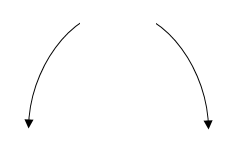
\includegraphics[width = 0.3\textwidth]{../Figures/polyEndBehaviorBB.png}\item 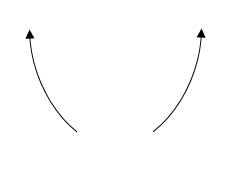
\includegraphics[width = 0.3\textwidth]{../Figures/polyEndBehaviorCB.png}\item 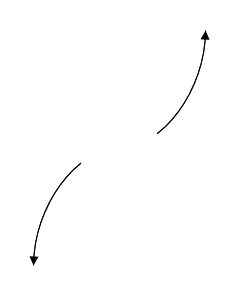
\includegraphics[width = 0.3\textwidth]{../Figures/polyEndBehaviorDB.png}\end{multicols}\item None of the above.
\end{enumerate} }
\litem{
Construct the lowest-degree polynomial given the zeros below. Then, choose the intervals that contain the coefficients of the polynomial in the form $ax^3+bx^2+cx+d$.\[ \frac{-1}{3}, 1, \text{ and } \frac{-2}{5} \]\begin{enumerate}[label=\Alph*.]
\item \( a \in [10, 17], b \in [3, 11], c \in [-9.39, -8.23], \text{ and } d \in [-0.3, 4.6] \)
\item \( a \in [10, 17], b \in [10, 23], c \in [-1.88, -0.96], \text{ and } d \in [-2.8, -0.2] \)
\item \( a \in [10, 17], b \in [-7, -3], c \in [-9.39, -8.23], \text{ and } d \in [-2.8, -0.2] \)
\item \( a \in [10, 17], b \in [-7, -3], c \in [-9.39, -8.23], \text{ and } d \in [-0.3, 4.6] \)
\item \( a \in [10, 17], b \in [-18, -11], c \in [-4.09, -2.6], \text{ and } d \in [-0.3, 4.6] \)

\end{enumerate} }
\end{enumerate}

\end{document}